% !TEX encoding   = UTF8
% !TEX spellcheck = ru_RU
% !TEX root = ../seminars.tex

%%==============================
\chapter{Модель вывода на экран}
%%==============================

%%=======================================
\section{Сборка библиотеки \texttt{FLTK}}
%%=======================================
\todo{\ldots добавить описание\ldots}



%%=============================
\section{Графические примитивы}
%%=============================
Рассмотрим пример из~\textbookref{раздела~12.7}, использующий графические классы.

\begin{figure}[ht]
    {\centering
        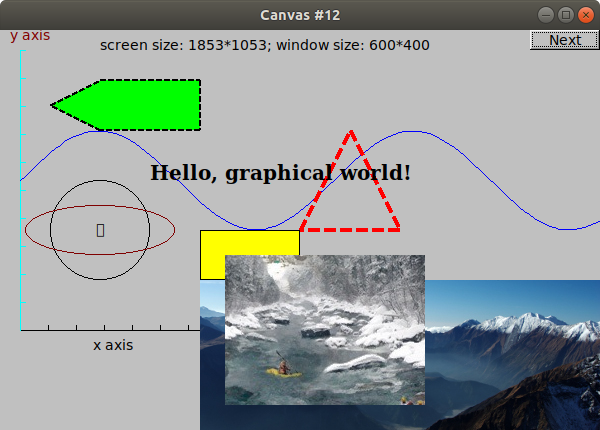
\includegraphics[width=0.6\textwidth]{images/shapes.png}

    }
    \caption{Окно программы c~графическими примитивами из~\textbookref{раздела~12.7}}
\end{figure}

\noindent Исходные файлы и проект программы размещены в~\href{\courserepourl}{репозитории}.

\begin{center}
    \code{projects/11/shape\_primitives}
\end{center}



%%=============
\paragraph{NB!}
%%=============
Использование директивы \code{using} приводит к~конфликту имён. В~системных графических библиотеках \name{Windows} определена функция \code{Rectangle}, а в~нашей графической библиотеке определён класс с~таким же именем. В~результате, компилятор обнаруживает неоднозначность определения имени.

Тем не~менее, поскольку все наши типы и функции размещены в~отдельном пространстве имён, следует просто уточнить, что мы имеем в~виду класс \code{Graph\_lib::Rectangle}.

\cppfile[firstline=1, lastline=10]{projects/11/shape_primitives/main.cpp}
\cppfile[firstline=12, lastline=21]{projects/11/shape_primitives/main.cpp}
\cpp`// ...`
\cppfile[firstline=48, lastline=51]{projects/11/shape_primitives/main.cpp}
\cpp`// ...`
\cppfile[firstline=113, lastline=113]{projects/11/shape_primitives/main.cpp}



%%=================================================
\section{Включение библиотеки \name{FLTK} в~проект}
%%=================================================
Рассмотрим внутренности проектного файла \code{CMakeLists.txt}, связанные с~добавлением внешней зависимости.

В~проект необходимо добавить файлы из~библиотеки \code{Graph\_lib}:

\cmakefile[firstline=22, lastline=23]{projects/11/shape_primitives/CMakeLists.txt}
\cmake'    # ...'
\cmakefile[firstline=25, lastline=28]{projects/11/shape_primitives/CMakeLists.txt}

\noindent которые будут подробно рассмотрены в~последующих \textbookref{главах} учебника. Классы этой библиотеки предоставляют нам сравнительно небольшой набор графических возможностей, реализованных на~основе библиотеки \name{FLTK}.

Система сборки \name{CMake} имеет механизмы поиска <<внешних>> библиотек в~системе. Это позволяет уменьшить зависимость описания проекта от~платформы, оставляя при~этом возможность вручную задать конкретные пути к~ним в~процессе конфигурации. Для поиска библиотеки \name{FLTK}, а также её зависимости "--- библиотеки более низкого уровня \name{OpenGL}, нужно добавить следующие строки:

\cmakefile[firstline=10, lastline=11]{projects/11/shape_primitives/CMakeLists.txt}

\noindent Флаг \code{REQUIRED} указывает, что без~данного компонента невозможна успешная сборка проекта. Таким образом, мы получаем более раннюю диагностику в~виде ошибки на~этапе конфигурирования.

\todo{\ldots добавить дальнейшее описание\ldots}

%Пути, дополнительные библиотеки и флаги компилятора зависят от платформы. Чтобы компилятор <<увидел>> заголовки (как правило, в угловых скобках), например:
%
%\begin{cppcode*}{linenos=false}
%#include <FL/Fl.H>
%#include <Graph_lib/Graph.h>
%\end{cppcode*}
%
%\noindent необходимо добавить пути (абсолютные или относительно проектного файла) к ним в стандартные пути поиска компилятора:
%
%%\jsfile[firstline=20, lastline=20]{projects/11/shape_primitives/shape_primitives.qbs}
%%\js'//      ...'
%%\jsfile[firstline=24, lastline=24]{projects/11/shape_primitives/shape_primitives.qbs}
%
%Заметим, что путь к заголовкам \name{FLTK} добавлен в системные пути. Дело в том, что иногда <<вылезают>> предупреждения компилятора, которые относятся к файлам сторонних библиотек, например, о неиспользуемых параметрах в функциях. Изменение внешнего кода является зачастую плохим решением (почему?). Если есть такое желание, следует внести вклад в разработку данной библиотеки. Современная система глобальной коммуникации легко позволяет оказать помощь разработчикам. Примером, могут служить проекты в \name{GitLab} или \name{GitHub}. Альтернатива "--- просто сообщить компилятору, что код подключается из внешней (системной) библиотеки. Тогда он не станет выдавать нам предупреждения, которые относятся к этим файлам.
%
%Аналогично, чтобы компоновщик смог найти дополнительные библиотеки, которые мы перечислили, необходимо добавить пути к ним, если они располагаются вне стандартных каталогов, как в нашем случае:
%
%\todo{добавить фрагмент проектного файла}
%%\jsfile[firstline=25, lastline=25]{projects/11/shape_primitives/shape_primitives.qbs}
%
%\noindent Также в \name{Windows} необходимо дать компоновщику опцию:
%
%\todo{добавить фрагмент проектного файла}
%%\jsfile[firstline=26, lastline=26]{projects/11/shape_primitives/shape_primitives.qbs}
%
%\noindent которая сообщает, что мы собираемся использовать оконный интерфейс.
%
%Ниже перечислены сторонние библиотеки (\textenglish{third-party libraries}), от которых, в свою очередь, зависит \name{FLTK} под \name{Windows}:
%
%\todo{добавить фрагмент проектного файла}
%%\jsfile[firstline=30, lastline=35]{projects/11/shape_primitives/shape_primitives.qbs}



%%================
\paragraph{P.\,S.}
%%================
Подводя итоги, перечислим необходимые в проекте компоненты для сборки программы, которая использует сторонние библиотеки:
\begin{itemfeature}
    \item пути к заголовкам;
    \item пути к библиотекам;
    \item дополнительные флаги компилятору;
    \item библиотеки;
    \item дополнительные флаги компоновщику.
\end{itemfeature}
Эти возможности присутствуют в каждой более-менее приличной среде разработки. Однако способы их добавления зависят от конкретной среды и могут сильно отличаться. Необходимо изучать соответствующие руководства.



%%%=========================================
%\paragraph{Проектный файл для \name{Linux}}
%%%=========================================
%тот же самый. Платформенно-зависимые свойства указаны в отдельном блоке:
%
%\jsfile[firstline=38, lastline=39]{projects/11/shape_primitives/shape_primitives.qbs}
%\js'//          ...'
%\jsfile[firstline=59, lastline=59]{projects/11/shape_primitives/shape_primitives.qbs}
%
%\noindent
%Инструкции читаются при условии, что целевая платформа "--- это \name{Linux}.
%
%Поправьте пути и имена библиотек в соответствии с версией \name{FLTK} на вашем компьютере. Ниже показано, как посмотреть флаги компилятора (\code{cxxflags}, \code{ldflags}), которые использует \name{FLTK}.



%%========================================================
\paragraph{Сборка в \name{Unix}-подобной командной среде.}
%%========================================================
Библиотека \name{FLTK} предоставляет удобную утилиту \code{fltk-config}, с помощью которой можно узнать необходимые настройки для сборки проекта, например:

\begin{consolecode}
$ fltk-config --cxxflags
-I/usr/local/include -I/usr/include/freetype2 -I/usr/include/libpng16 \
-D_LARGEFILE_SOURCE -D_LARGEFILE64_SOURCE -D_THREAD_SAFE -D_REENTRANT
$ fltk-config --ldflags
-L/usr/local/lib -lfltk -lXrender -lXcursor -lXfixes -lXext -lXft \
-lfontconfig -lXinerama -lpthread -ldl -lm -lX11
\end{consolecode}

\noindent и собрать исполняемый модуль программы:

\begin{consolecode}
$ g++ -o bin/shapes -std=c++14 -pedantic $(fltk-config --cxxflags) \
  projects/11/shape_primitives/main.cpp lib/Graph_lib/*.cpp \
  $(fltk-config --use-images --ldflags)
\end{consolecode}

Обратите внимание на использование конструкции \code{\$(command)} "--- аналог косых кавычек \code{`command`}. Командная среда вначале выполняет команду \code{command}, а затем подставляет на её место результат (то, что вывелось бы на экран) и запускает образовавшуюся в итоге команду.

Стандартный способ узнать возможности какой-либо утилиты "--- вызвать справку:
\console`$ fltk-config --help`%$

Теперь можно запустить нашу программу:
\console`$ bin/shapes`%$



%%==========================
\section{Элементы геометрии}\label{sect:geomelems}
%%==========================
Напишем ряд вспомогательных функций. Чтобы не загромождать основную программу и в дальнейшем иметь возможность использовать код повторно, разместим их в отдельном модуле (\code{lib/poly}): \code{poly.h}/\code{poly.cpp}.

Функция \code{regular\_polygon()} возвращает список вершин правильного \code{n}-угольника с центром в точке \code{center}, радиусом описанной окружности \code{radius} и начальным положением (углом) \code{angle} первой вершины, отсчитывая от оси X. Последний параметр позволяет задать необходимую ориентацию на плоскости нашего многоугольника. Положительное значение угла задаёт вращение против часовой стрелки. По умолчанию значение этого угла равно \code{0}.

\cppfile[firstline=17, lastline=32]{projects/lib/poly/poly.cpp}

\noindent
\parbox[c]{0.65\textwidth}{\parindent=1.25cm%
Изменение координат точки при вращении можно выразить через поворот самой системы координат:
\[
  \left\{ \begin{array}{l}
    x\prime = \phantom{-}x\cos\alpha + y\sin\alpha, \\
    y\prime =           -x\sin\alpha + y\cos\alpha.
  \end{array}\right.
\]
Используя эти соотношения, функция \code{rotated()} выполняет поворот точки \code{point} на угол \code{angle} относительно центра вращения \code{center} и возвращает новую точку. По умолчанию центр вращения расположен в начале координат.
}\hfill\parbox[c]{0.35\textwidth}{%
\begin{center}\begin{tikzpicture}[>=Stealth, very thick]
  \draw[help lines, step=.5cm] (-2, -1) grid (2.5, 2.5);
  \draw[->] (-0.5, 0) -- (2, 0) node[at end, below=3pt, fill=white] {\(x\)};
  \draw[->] (0, -0.5) -- (0, 2) node[at end, right=3pt, fill=white] {\(y\)};
  \draw[->, blue] (1.5, 0) arc [start angle=0, end angle=30, radius=1.5cm] node[midway, right=2pt, color=blue, fill=white] {\(\alpha\)};
  \draw[->, blue, rotate=30] (-0.5, 0) -- (2, 0) node[at end, above=1pt, color=blue, fill=white] {\(x\prime\)};
  \draw[->, blue, rotate=30] (0, -0.5) -- (0, 2) node[at end, left=1pt, color=blue, fill=white] {\(y\prime\)};
\end{tikzpicture}\end{center}
}% parbox

\cppfile[firstline=7, lastline=15]{projects/lib/poly/poly.cpp}

Функция \code{lerp()} добавлена в стандартную библиотеку \lang{C++20}. Она выполняет линейную интерполяцию между \(a\) и \(b\) для параметра \(t\) (или экстраполяцию, если \(t \notin [0, 1]\)).

\cppfile[firstline=30, lastline=30]{projects/lib/poly/poly.h}

Будет удобна ещё одна простая функция \code{append()}, которая добавит точки из списка в замкнутую ломаную \code{Closed\_polyline} из нашей графической библиотеки.

\cppfile[firstline=34, lastline=38]{projects/lib/poly/poly.cpp}

\noindent Здесь функция \code{as\_point()} преобразует вещественный радиус-вектор \code{Vec2d} в экранную точку \code{Point}, выполняя округление до целых значений по правилам математики.

\cppfile[firstline=32, lastline=35]{projects/lib/poly/poly.h}

\noindent Такое округление улучшает точность отрисовки линий на экране.



%%================
\section{Фракталы}
%%================
\emph{Фракталом} называется структура, состоящая из частей, которые в каком-то смысле подобны целому. Этот существенный отличительный признак наблюдается в эксперименте: фрактал выглядит одинаково, в каком бы масштабе его ни наблюдать. Взять хотя бы некоторые прекрасные кучевые облака. Они состоят из огромных <<горбов>>, на которых возвышаются <<горбы>> поменьше, на тех "--- <<горбы>> ещё меньше и т.д. вплоть до самого малого масштаба, который вы в состоянии разрешить.

\begin{figure}[ht]
    {\centering
        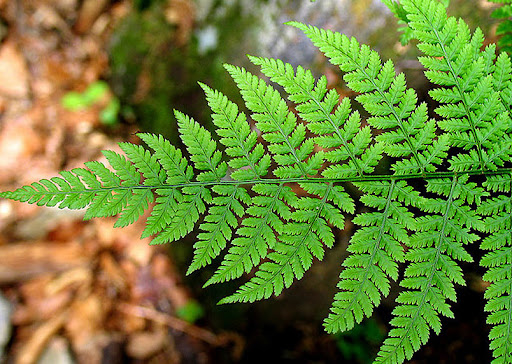
\includegraphics[height=0.26\textwidth]{images/fern.jpg}\hfil
        
\includegraphics[height=0.26\textwidth]{images/clouds.jpg}\hfil
        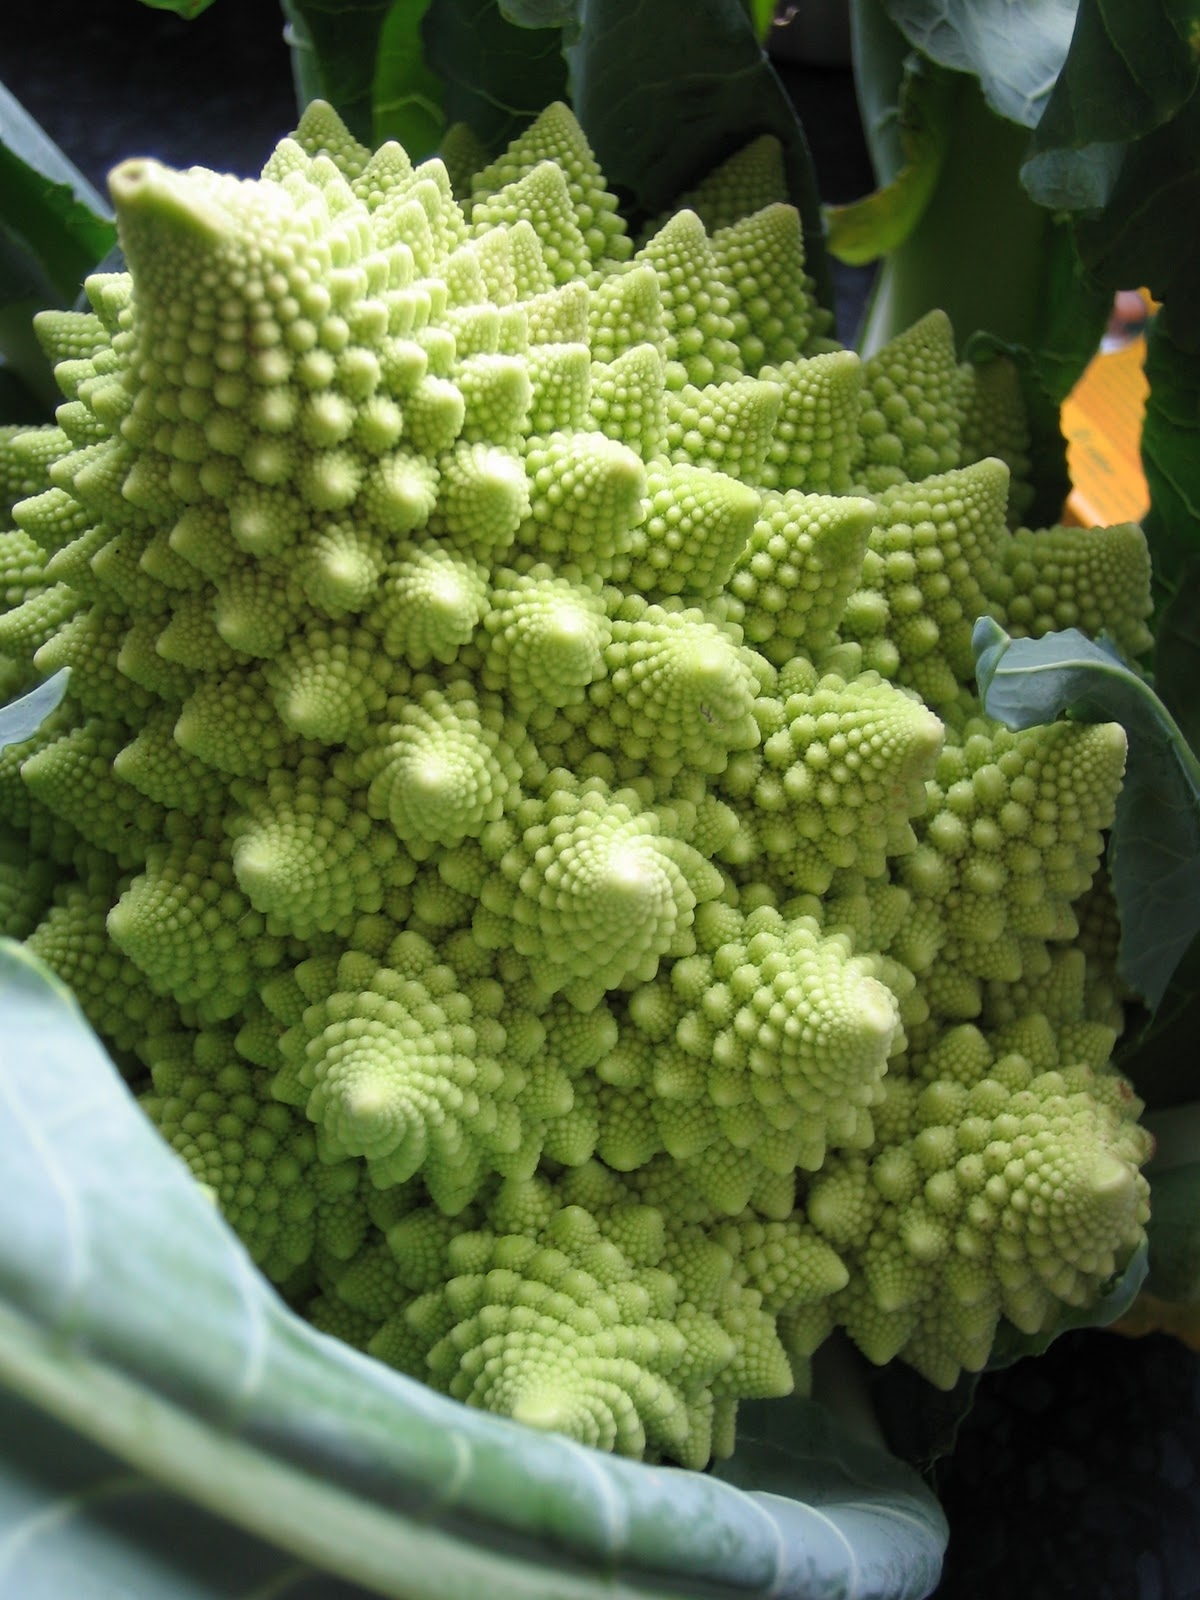
\includegraphics[height=0.26\textwidth]{images/romanesco_broccoli.jpg}

    }
    \caption{Примеры фракталов в природе}
\end{figure}



%%========================
\paragraph{Снежинка Коха,}
%%========================
построенная в виде замкнутой кривой на базе равностороннего треугольника, впервые была описана шведским математиком \href{https://ru.wikipedia.org/wiki/Кох,_Нильс_Фабиан_Хельге_фон}{Хельге фон Кохом} в 1904 году. В некоторых работах она получила название «остров Коха».

Доказано, что эта фрактальная кривая обладает рядом любопытных свойств. К примеру, длина её периметра равна бесконечности, что, однако, не мешает охватывать конечную площадь, величина которой равна \(\frac{8}{5}\) площади базового треугольника.

\begin{figure}[ht]
    {\centering
        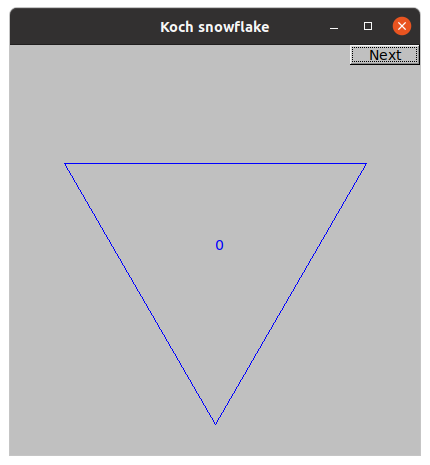
\includegraphics[width=0.3\textwidth]{images/koch_snowflake_n=0.png}\hfil
        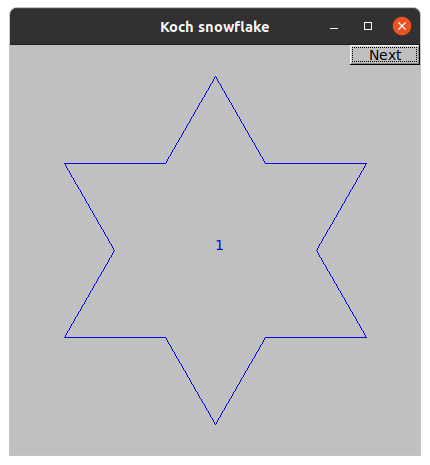
\includegraphics[width=0.3\textwidth]{images/koch_snowflake_n=1.png}\hfil
        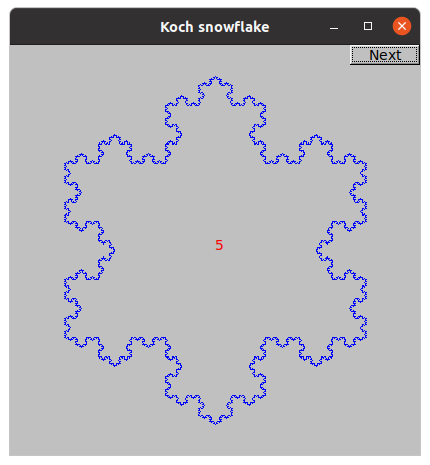
\includegraphics[width=0.3\textwidth]{images/koch_snowflake_n=5.png}

    }
    \caption{Снежинка Коха}
    \label{fig:kochshowflake}
\end{figure}

Построение кривой Коха начинается с прямолинейного отрезка единичной длины. Этот исходный отрезок называется \emph{затравкой} и может быть заменён каким-нибудь многоугольником, например, равносторонним треугольником или квадратом. Затравка "--- это \(0\)-е поколение кривой Коха. Далее, каждое звено затравки заменяется \emph{образующим элементом} "--- отрезок делится на 3 равные части и средняя часть заменяется равносторонним треугольником, у которого удалено основание (рисунок~\ref{fig:kochshowflake}).

Шаг этого алгоритма можно выразить следующим образом, используя ранее приведённые вспомогательные функции:

\cppfile[firstline=24, lastline=38]{projects/11/koch_snowflake/main.cpp}

Контейнер \code{std::list} представляет собой двусвязный список. Обойти его элементы можно используя итераторы "--- обобщённый аналог указателей. Они будут рассмотрены в \textbookref{главе~20} учебника. Список передаётся по rvalue-ссылке, которая позволяет избежать ненужного копирования объекта. Подробнее об этих ссылках и перемещении (\code{std::move}) мы узнаем в \textbookref{главе~18} учебника.

Вариант рисования снежинки Коха на базе правильного \code{n}-угольника в окне шириной~\code{w} средствами нашей библиотеки \code{Graph\_lib} можно записать так:

\cppfile[firstline=52, lastline=81]{projects/11/koch_snowflake/main.cpp}

Мы добавили текстовую метку в центре фигуры, показывающую номер шага алгоритма. И также учли, что дальнейшее измельчение кривой бессмысленно, если длина ребра становится менее~\(1\) пикселя. Функцию \code{max\_edge\_length()} предлагаем реализовать самостоятельно.

\textbf{NB!} Обратите особое внимание, что замкнутая ломаная создаётся в теле цикла каждый раз заново. Дело в том, что \code{Graph\_lib} не предоставляет удобного способа добавления новых точек в середину кривой. Мы вынуждены откреплять нашу кривую от окна в конце итерации, чтобы избежать отрисовки несуществующего объекта.


%=================
% !TEX encoding   = UTF8
% !TEX spellcheck = ru_RU
% !TEX root = ../seminars.tex

%%=================================
\section{Правильные многоугольники}
%%=================================
Нарисуем ряд вложенных правильных многоугольников из~упражнения~11 \textbookref{главы~12}.

\begin{figure}[ht]
  {\centering
    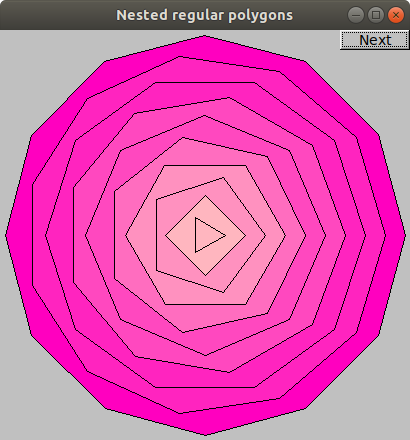
\includegraphics[height=0.3\textwidth]{images/regular_polygons.png}

  }
  \caption{Вложенные правильные многоугольники}
  \label{fig:regpoly}
\end{figure}

Покажем лишь ключевой фрагмент кода. Напомним, что функция \code{regular\_polygon()} вычисляет вершины правильного многоугольника и была представлена ранее в~разделе~\ref{sect:geomelems}.

\cppfile[firstline=19, lastline=45]{projects/11/regular_polygons.cpp}

Класс \code{Vector\_ref} рассматривается в~\textbookref{главе~13} и удобен для~хранения множества неименованных объектов. Многоугольники рисуются с~использованием вращательной симметрии и раскрашиваются в~оттенки пурпурного (см. диаграмму цветов из~\textbookref{главы~13}). Результат работы программы показан на~рисунке~\ref{fig:regpoly}.



%%====================
\section{Суперэллипсы}
%%====================
Суперэллипс, также известный как кривая Лямэ, названная в~честь \href{https://en.wikipedia.org/wiki/Gabriel_Lam\%C3\%A9}{Габриэля Лямэ}, "--- замкнутая кривая, которая как и эллипс обладает большой и малой полуосями, а также симметрией относительно них, но в~общем случае другой формой.

\begin{figure}[ht]
  {\centering
    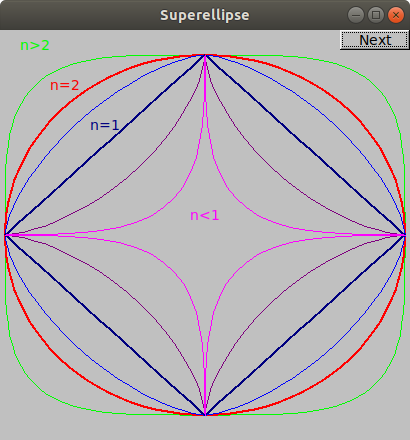
\includegraphics[height=0.3\textwidth]{images/superellipse.png}

  }
  \caption{Суперэллипсы}
  \label{fig:superellipse}
\end{figure}

В~декартовой системе координат суперэллипс в~обобщённом виде задаётся следующим соотношением:
\[
  \left| \frac{x}{a} \right|^m + \left| \frac{y}{b} \right|^n = 1;\quad m, n > 0.
\]

В~параметрическом виде, где параметр~\(t\) не~имеет никакой геометрической интерпретации, кривая выражается системой уравнений:
\begin{equation}
  \label{eq:superellipse}
  \left\{\begin{array}{l}
    x(t) = a\,\mathrm{sign}(\cos t) \cdot |\cos t|^{\frac{2}{m}},\\
    y(t) = b\,\mathrm{sign}(\sin t) \cdot |\sin t|^{\frac{2}{n}};
  \end{array}\right.
  \quad 0 \leqslant t \leqslant 2\pi.
\end{equation}

Функция, добавляющая точки, лежащие на~суперэллипсе, по~формуле~(\ref{eq:superellipse}), приведена ниже:

\cppfile[firstline=20, lastline=35]{projects/11/superellipse.cpp}

Функцию, определяющую знак числа, можно написать таким образом:

\cppfile[firstline=18, lastline=18]{projects/11/superellipse.cpp}

Ключевой фрагмент функции \code{main()} для~рисования нескольких вложенных суперэллипсов из~упражнения~12 \textbookref{главы~12}:

\cppfile[firstline=40, lastline=54]{projects/11/superellipse.cpp}

Мы уверены, что вы сможете самостоятельно добавить текстовые метки (подписи) к~кривым и раскрасить их, например, как на~рисунке~\ref{fig:superellipse}.

%=================



%%================
\WhatToReadSection
%%================
\textcite{Stroustrup:2016:ru}: \textbf{глава~13}



%%===============
\ExercisesSection
%%===============
\begin{exercise}
\item Выполните упражнения из \textbookref{главы~12} учебника.

\item Постройте так называемую антиснежинку Коха. Алгоритм генерирования заключается в вырезании на каждом этапе всё новых и новых треугольников из исходного многоугольника. Иными словами, рёбра базовой формы модифицируются внутрь, а не наружу. В результате полученная фигура охватывает бесконечное множество несвязанных областей.

\begin{figure}[ht]
  {\centering
    
\includegraphics[height=0.2\textwidth]{images/koch_curve_85_degrees.png}

  }
  \caption{Фрактал Цезаро "--- вариант кривой Коха с углом между \(60^{\circ}\) и \(90^{\circ}\) (\(85^{\circ}\))}
\end{figure}

\item Нарисуйте дракона Хартера, также известного как дракона Хартера--Хейтуэя. Он был впервые исследован физиками \name{NASA} "--- Джоном Хейтуэем (John Heighway), Брюсом Бэнксом (Bruce Banks), и Вильямом Хартером (William Harter). В 1967 году описан Мартином Гарднером в колонке «Математические игры» журнала <<\textenglish{Scientific American}>>. Многие из свойств фрактала были описаны Чендлером Дэвисом (Chandler Davis) и Дональдом Кнутом.

\begin{figure}[ht]
  \begin{center}
    \fbox{\begin{minipage}{0.4\textwidth}
      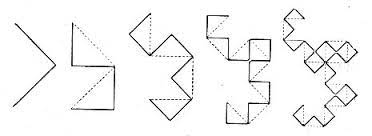
\includegraphics[width=\textwidth]{images/harter-heighway_dragon_steps-1.jpg}\\
      
\includegraphics[width=\textwidth]{images/harter-heighway_dragon_steps-2.png}
    \end{minipage}}
    \hfil
    \fbox{\begin{minipage}{0.25\textwidth}
      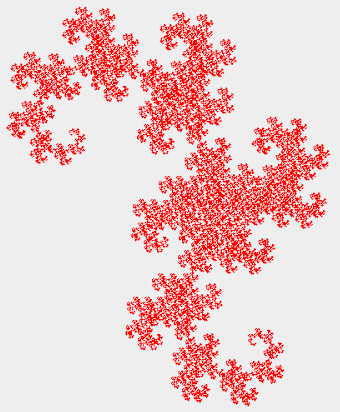
\includegraphics[width=\textwidth]{images/harter-heighway_dragon.png}
    \end{minipage}}
  \end{center}
  \caption{Дракон Хартера--Хейтуэя}
\end{figure}

\end{exercise}
